\subsection{Image Analysis}
	\gls{ia} is the use of various techniques, such as pattern recognition, geometry calculations, and signal processing, to extract information from digital images. Image processing is the application of various processes on an image to change or enhance its appearance. In practice, the processing stage normally comes before the analysis stage as a way of simplifying the image prior to analysis in order to maximize the likelihood of obtaining usable data.
	\subsubsection{Digital Camera Operation}
		A digital camera operates by capturing visible light reflected by objects onto the camera’s sensor. The light must travel from the object through a convex focusing lens which refracts the light onto a corresponding point on the sensor.
		\begin{figure}[h!]
			\centering
			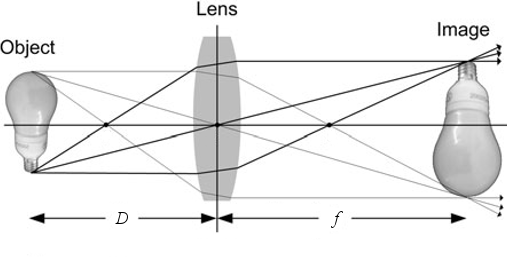
\includegraphics[width=10cm]{../images/camera_bulb.PNG}
			\caption{Diagram of camera and lens operation \citep{introtoprocessing}}
			\label{fig:camera_diagram}
		\end{figure}
		\\
		The distance between where light enters the lens and the point at which it is no longer diffused is known as the focal length, marked $f$ in figure \ref{fig:camera_diagram}. This point can be adjusted by changing the optical characteristics of the lens so that the refracted light hits the sensor to create a sharply focused image.
		\\\\
		A camera’s sensor is made up of an array of photosensitive cells capable of collecting light and generating an integer value based on the brightness and colour of the received light. The microprocessor inside the camera takes these values and converts them into the image data, sometimes taking an average of the surrounding values to better understand the light as it was captured. Each of the cells in the camera’s sensor equates to a single pixel in the final image. For example, a camera with a sensor made up of 1920 cells across by 1080 down (otherwise known as a 2 megapixel sensor) produces an image 1920 pixels wide and 1080 high. The larger the physical size of the sensor, the more cells it can contain resulting in a higher quality image.
		\\\\
		Image processing is the manipulation of these integer values to adjust the visual appearance of the image for either artistic or scientific purposes. Image analysis is the comparison of these values either to their neighbours or in clusters to locate features, produce measurements, or for other purposes within the context of the image.
	\subsubsection{Lighting Conditions}
		When capturing images to be analysed, it is important to have good lighting conditions so that none of the required detail is lost \citep{introtoprocessing}. If the image is captured in unsuitable conditions, such as low light, then this can seriously affect the outcome of subsequent analysis. 
		\\\\
		Certain image processing techniques, such post-processing images captured as Camera RAW files, can help ameliorate poor lighting conditions though this is not foolproof and it is always better to capture a well-lit image. Figure \ref{fig:illumination} shows the effects that different lighting angles have on a subject.
		\begin{figure}[h!]
			\centering
			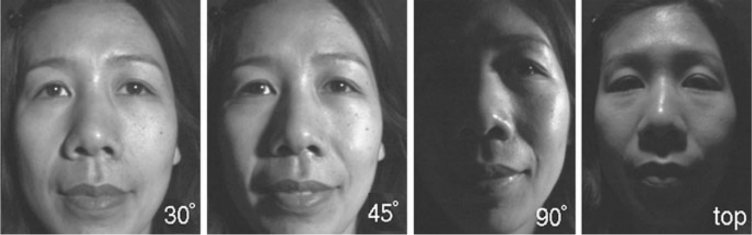
\includegraphics[width=\linewidth]{../images/face_illumination.png}
			\caption[]{The effects of different lighting conditions on a face \citep{introtoprocessing}}
			\label{fig:illumination}
		\end{figure}\\
		It can be seen that the situation which highlights the most detail is when the light source is close to being in front of the subject matter. Such lighting reduces the amount of image processing required before analysing and produces the largest amount of usable data. In the context of this project many smartphones also have an integral flash function which means the user can correctly light their image in sub-optimal lighting conditions where required detail may otherwise be lost.
	\subsubsection{Usages}
		Image processing and image analysis have been applied to multiple areas with its value and effectiveness rapidly improving alongside advances in camera technology and computing power. These applications range from facial recognition in social media uploads \citep{zuckerberg2011tagging} to the utilisation of satellite imagery to track the changing shape of coastlines \citep{costalimagery}.
		\begin{figure}[h!]
			\centering
			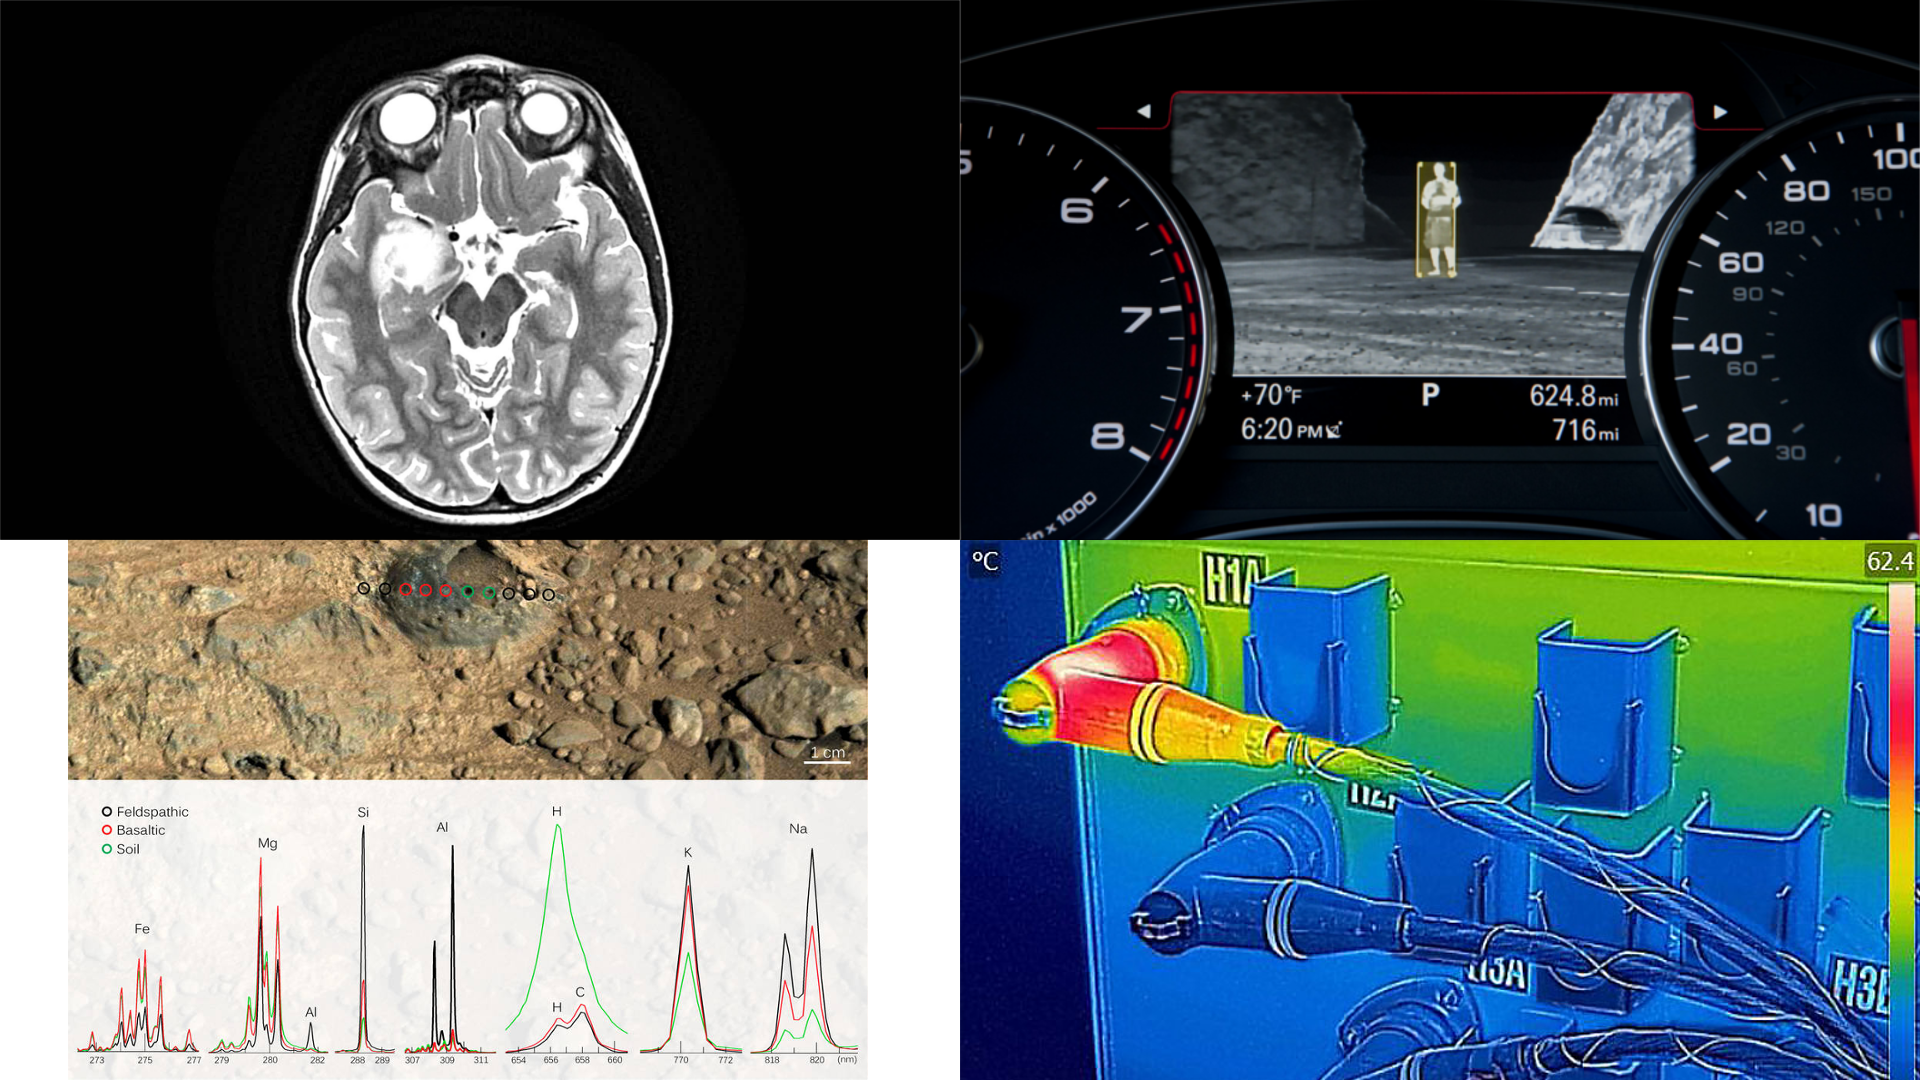
\includegraphics[width=15cm]{../images/4panel.png}
			\caption[Uses of image analysis]{Uses of image analysis, from top left clockwise: An MRI brain scan, automotive night vision with pedestrian recognition, infrared image taken with a smartphone, chemical rock analysis from mars}
			\label{fig:analysis_uses}
		\end{figure}
		\paragraph{Medical}
			This is arguably one of the most important uses of IA. Advances in medical imaging have reduced costs, diagnosis time and patient recovery time while improving the ability to localise and personalise treatments \citep{esfmedical}. Major uses of IA in medical applications are the use of Magnetic Resonance Imaging (MRI) and Computerised Topography Scanning (CT Scan) to create detailed images of the human body and identify illness before obvious symptoms appear. This is shown top left in Figure \ref{fig:analysis_uses}.
		\paragraph{Transport}
			Image analysis has been included in the consumer automotive market on various models since 2004 when Honda introduced a thermographic night vision camera with automatic pedestrian detection on their Legend model \citep{hondanightvision}. Other manufacturers, including Audi, have since introduced similar technology and their implementation can be seen top right in Figure \ref{fig:analysis_uses}. Since this initial use many other vehicle manufacturers have included functionality based on image analysis expanding its use into areas such as the automatic recognition of speed limit signs, lane departure warning systems, and automatic braking systems based on hazard recognition.
		\paragraph{Engineering}
			The use of image analysis in engineering has helped to create more stable and efficient structures, in bridges and skyscrapers for example, by looking at the materials used in their construction \citep{concreteanalysis} and monitoring their stresses and potential areas of weakness \citep{bridgecables}. Today advances in mobile computing have allowed engineers to routinely use IA while on site and some application vendors target their products at an engineering sector by improving their durability and integrating features such as infrared imaging \citep{catphone}, the output of which can be seen lower right in Figure \ref{fig:analysis_uses}.
		\paragraph{Space}
			While some industries make use of satellite imagery to monitor 
			chan-ges to our own planet, agencies such as NASA and ESA use image analysis to look at other planets and celestial bodies. The Martian rover, Curiosity, uses multiple cameras for navigation, hazard avoidance, and scientific imaging with the images streamed back to Earth for detailed analysis. Major uses of such extraterrestrial images include the identification of geological formations and their likely composition \citep{curiositysand, curiositygravel} and the location and identification of chemicals using the analysis tools such as ”ChemCam” \citep{curiosityhydrogen}, which can be seen lower left in Figure \ref{fig:analysis_uses}.